\documentclass[12pt]{article}
%\usepackage{scrextend}
%\usepackage{lipsum}

%\deffootnote[10pt]{10pt}{10pt}{\makebox[10pt][l]{\thefootnotemark\hspace{10pt}}}

\usepackage{footmisc}

\usepackage[nocompress]{cite} %makes sure multiple citations are ordered correctly, e..g [5, 17, 20]

\usepackage{amsmath,amssymb,graphicx,booktabs,multirow,mathtools,mathrsfs}
\usepackage{caption,subcaption,float,hyperref}
\usepackage{float, afterpage}
\usepackage[toc,page]{appendix}
\usepackage{breakurl}

%%%%%%%%% HYPERREF COLORS %%%%%%%%%%%%
\usepackage{xcolor}
\definecolor{warmblue}{RGB}{66,106,181}
\hypersetup{
colorlinks,
linkcolor=warmblue,
urlcolor=warmblue,
citecolor=warmblue
}

%%%%%%%%%% HYPHENATION %%%%%%%%%%%%%%
\usepackage[british]{babel}
\hyphenation{di-men-sio-nal}
%%%%%%%%%% HYPHENATION %%%%%%%%%%%%%%

%%%%%%%%%%%% HEADERS %%%%%%%%%%%%%%%
\usepackage{fancyhdr}
\pagestyle{fancy}
\fancyhf{}
\fancyhead[R]{\nouppercase\rightmark} % 1. sectionname
\fancyfoot[C]{\thepage}
\fancypagestyle{plain}{%
  \fancyhf{}%
  \renewcommand{\headrulewidth}{0pt}%
  }
%%%%%%%%%%%% HEADERS %%%%%%%%%%%%%%%

%%%%%%%%%%% TROUSERS SYMBOLS %%%%%%%%%%
\newcommand\xBone{\raisebox{-1.2ex}{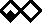
\includegraphics[height=3.5ex]{B1symb}}}
\newcommand\Bone{{\mathchoice{\xBone}{\xBone}{\hbox{\scriptsize\xBone}}{\hbox{\tiny\xBone}}}}
\newcommand\xBtwo{\raisebox{-1.2ex}{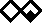
\includegraphics[height=3.5ex]{B2symb}}}
\newcommand\Btwo{{\mathchoice{\xBtwo}{\xBtwo}{\hbox{\scriptsize\xBtwo}}{\hbox{\tiny\xBtwo}}}}
\newcommand\xULDone{\raisebox{-1.2ex}{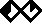
\includegraphics[height=3.5ex]{ULD1symb}}}
\newcommand\ULDone{{\mathchoice{\xULDone}{\xULDone}{\hbox{\scriptsize\xULDone}}{\hbox{\tiny\xULDone}}}}
\newcommand\xULDtwo{\raisebox{-1.2ex}{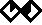
\includegraphics[height=3.5ex]{ULD2symb}}}
\newcommand\ULDtwo{{\mathchoice{\xULDtwo}{\xULDtwo}{\hbox{\scriptsize\xULDtwo}}{\hbox{\tiny\xULDtwo}}}}
\newcommand\xMLone{\raisebox{-1.2ex}{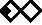
\includegraphics[height=3.5ex]{ML1symb}}}
\newcommand\MLone{{\mathchoice{\xMLone}{\xMLone}{\hbox{\scriptsize\xMLone}}{\hbox{\tiny\xMLone}}}}
\newcommand\xMLtwo{\raisebox{-1.2ex}{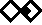
\includegraphics[height=3.5ex]{ML2symb}}}
\newcommand\MLtwo{{\mathchoice{\xMLtwo}{\xMLtwo}{\hbox{\scriptsize\xMLtwo}}{\hbox{\tiny\xMLtwo}}}}
\newcommand\xMRone{\raisebox{-1.2ex}{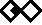
\includegraphics[height=3.5ex]{MR1symb}}}
\newcommand\MRone{{\mathchoice{\xMRone}{\xMRone}{\hbox{\scriptsize\xMRone}}{\hbox{\tiny\xMRone}}}}
\newcommand\xMRtwo{\raisebox{-1.2ex}{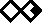
\includegraphics[height=3.5ex]{MR2symb}}}
\newcommand\MRtwo{{\mathchoice{\xMRtwo}{\xMRtwo}{\hbox{\scriptsize\xMRtwo}}{\hbox{\tiny\xMRtwo}}}}
\newcommand\xLRDone{\raisebox{-1.2ex}{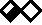
\includegraphics[height=3.5ex]{LRD1symb}}}
\newcommand\LRDone{{\mathchoice{\xLRDone}{\xLRDone}{\hbox{\scriptsize\xLRDone}}{\hbox{\tiny\xLRDone}}}}
\newcommand\xLRDtwo{\raisebox{-1.2ex}{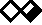
\includegraphics[height=3.5ex]{LRD2symb}}}
\newcommand\LRDtwo{{\mathchoice{\xLRDtwo}{\xLRDtwo}{\hbox{\scriptsize\xLRDtwo}}{\hbox{\tiny\xLRDtwo}}}}
\newcommand\xURDone{\raisebox{-1.2ex}{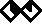
\includegraphics[height=3.5ex]{URD1symb}}}
\newcommand\URDone{{\mathchoice{\xURDone}{\xURDone}{\hbox{\scriptsize\xURDone}}{\hbox{\tiny\xURDone}}}}
\newcommand\xURDtwo{\raisebox{-1.2ex}{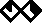
\includegraphics[height=3.5ex]{URD2symb}}}
\newcommand\URDtwo{{\mathchoice{\xURDtwo}{\xURDtwo}{\hbox{\scriptsize\xURDtwo}}{\hbox{\tiny\xURDtwo}}}}
\newcommand\xLLDone{\raisebox{-1.2ex}{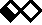
\includegraphics[height=3.5ex]{LLD1symb}}}
\newcommand\LLDone{{\mathchoice{\xLLDone}{\xLLDone}{\hbox{\scriptsize\xLLDone}}{\hbox{\tiny\xLLDone}}}}
\newcommand\xLLDtwo{\raisebox{-1.2ex}{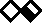
\includegraphics[height=3.5ex]{LLD2symb}}}
\newcommand\LLDtwo{{\mathchoice{\xLLDtwo}{\xLLDtwo}{\hbox{\scriptsize\xLLDtwo}}{\hbox{\tiny\xLLDtwo}}}}
\newcommand\xTLone{\raisebox{-1.2ex}{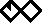
\includegraphics[height=3.5ex]{TL1symb}}}
\newcommand\TLone{{\mathchoice{\xTLone}{\xTLone}{\hbox{\scriptsize\xTLone}}{\hbox{\tiny\xTLone}}}}
\newcommand\xTLtwo{\raisebox{-1.2ex}{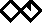
\includegraphics[height=3.5ex]{TL2symb}}}
\newcommand\TLtwo{{\mathchoice{\xTLtwo}{\xTLtwo}{\hbox{\scriptsize\xTLtwo}}{\hbox{\tiny\xTLtwo}}}}
\newcommand\xTRone{\raisebox{-1.2ex}{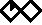
\includegraphics[height=3.5ex]{TR1symb}}}
\newcommand\TRone{{\mathchoice{\xTRone}{\xTRone}{\hbox{\scriptsize\xTRone}}{\hbox{\tiny\xTRone}}}}
\newcommand\xTRtwo{\raisebox{-1.2ex}{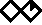
\includegraphics[height=3.5ex]{TR2symb}}}
\newcommand\TRtwo{{\mathchoice{\xTRtwo}{\xTRtwo}{\hbox{\scriptsize\xTRtwo}}{\hbox{\tiny\xTRtwo}}}}
\newcommand\xPOD{\raisebox{-1.2ex}{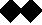
\includegraphics[height=3.5ex]{PODsymb}}}
\newcommand\POD{{\mathchoice{\xPOD}{\xPOD}{\hbox{\scriptsize\xPOD}}{\hbox{\tiny\xPOD}}}}
\newcommand\xLL{\raisebox{-1.2ex}{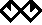
\includegraphics[height=3.5ex]{LLsymb}}}
\newcommand\LL{{\mathchoice{\xLL}{\xLL}{\hbox{\scriptsize\xLL}}{\hbox{\tiny\xLL}}}}
\newcommand\xRL{\raisebox{-1.2ex}{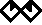
\includegraphics[height=3.5ex]{RLsymb}}}
\newcommand\RL{{\mathchoice{\xRL}{\xRL}{\hbox{\scriptsize\xRL}}{\hbox{\tiny\xRL}}}}
\newcommand\xSides{\raisebox{-1.2ex}{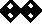
\includegraphics[height=3.5ex]{Ssymb}}}
\newcommand\Sides{{\mathchoice{\xSides}{\xSides}{\hbox{\scriptsize\xSides}}{\hbox{\tiny\xSides}}}}
\newcommand\xCausal{\raisebox{-1.2ex}{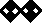
\includegraphics[height=3.5ex]{Csymb}}}
\newcommand\Causal{{\mathchoice{\xCausal}{\xCausal}{\hbox{\scriptsize\xCausal}}{\hbox{\tiny\xCausal}}}}
\newcommand\xNFone{\raisebox{-1.2ex}{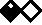
\includegraphics[height=3.5ex]{NF1symb}}}
\newcommand\NFone{{\mathchoice{\xNFone}{\xNFone}{\hbox{\scriptsize\xNFone}}{\hbox{\tiny\xNFone}}}}
\newcommand\xFPUone{\raisebox{-1.2ex}{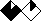
\includegraphics[height=3.5ex]{FPU1symb}}}
\newcommand\FPUone{{\mathchoice{\xFPUone}{\xFPUone}{\hbox{\scriptsize\xFPUone}}{\hbox{\tiny\xFPUone}}}}
\newcommand\xFPUtwo{\raisebox{-1.2ex}{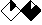
\includegraphics[height=3.5ex]{FPU2symb}}}
\newcommand\FPUtwo{{\mathchoice{\xFPUtwo}{\xFPUtwo}{\hbox{\scriptsize\xFPUtwo}}{\hbox{\tiny\xFPUtwo}}}}
\newcommand\xFPVone{\raisebox{-1.2ex}{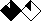
\includegraphics[height=3.5ex]{FPV1symb}}}
\newcommand\FPVone{{\mathchoice{\xFPVone}{\xFPVone}{\hbox{\scriptsize\xFPVone}}{\hbox{\tiny\xFPVone}}}}
\newcommand\xFPVtwo{\raisebox{-1.2ex}{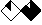
\includegraphics[height=3.5ex]{FPV2symb}}}
\newcommand\FPVtwo{{\mathchoice{\xFPVtwo}{\xFPVtwo}{\hbox{\scriptsize\xFPVtwo}}{\hbox{\tiny\xFPVtwo}}}}

%%%%%%%%%%% ABBREVIATED COMMANDS %%%%%%%%%%
%%%%%% STANDARD DEFINITIONS:
\newcommand{\be}{\begin{equation}}
\newcommand{\ee}{\end{equation}}
\newcommand{\bal}{\begin{aligned}}
\newcommand{\eal}{\end{aligned}}
\newcommand{\nn}{\nonumber\\}
\newcommand{\mm}{\medmath}
\newcommand{\s}{\scriptstyle}
\newcommand{\mb}[1]{\marginpar{\texttt{#1}}}
\newcommand*\dAlembert{\mathop{}\!\mathbin\Box}
%%%%%%% LOCAL DEFINITIONS:
\newcommand{\bth}{\boldsymbol\theta}
\newcommand{\bes}{\begin{split}}
\newcommand{\ees}{\end{split}}
\def\bea{\begin{equation}\begin{aligned}}
\def\eea{\end{aligned}\end{equation}}
%\newcommand{\Log}{\textrm{Ln}}
\DeclareMathOperator{\Log}{Ln}
\DeclareMathOperator{\csch}{csch}
\newcommand{\sgn}{\textrm{sgn}}
\newcommand{\vecj}{\mathbf{j}}
\newcommand{\veck}{\mathbf{k}}
\newcommand{\vecq}{\mathbf{q}}
\newcommand{\veca}{\mathbf{a}}
\newcommand{\vecb}{\mathbf{b}}
\newcommand{\vecx}{\mathbf{x}}
\newcommand{\vecy}{\mathbf{y}}
\newcommand{\sech}{\mathrm{sech}}
\renewcommand{\Re}{\mathrm{Re}}
\renewcommand{\Im}{\mathrm{Im}}
\newcommand{\MBEDIT}[1]{}
%\newcommand{\colrulespace}{\noalign{\smallskip}\colrule\noalign{\smallskip}}
%%%%%%%%%% ABBREVIATED COMMANDS %%%%%%%%%%

\begin{document}

So far, the spacetimes we have considered have all been globally hyperbolic. Global hyperbolicity is an important property in the usual construction of quantum field theory in flat and curved spacetime, since it guarantees that linear hyperbolic equations such as the Klein-Gordon equation admit a well-posed initial value problem and have well defined global advanced and retarded propagators~\cite{leray1953hyperbolic,hawking1975large}. Yet there are situations in which one may like to consider spacetimes that fall short of the criterion. Anti de Sitter space is perhaps the most famous example of a spacetime that is not globally hyperbolic and yet of tremendous interest in the context of the gauge-gravity (AdS/CFT) correspondence~\cite{Avis:1977yn}. Another case, the one that we will pay attention to in this chapter, is that of spacetimes experiencing topology-change. Such spacetimes cannot be globally hyperbolic: a globally hyperbolic Lorentzian manifold must be homeomorphic to $\Sigma\times\mathbb R$ ~\cite{Geroch:1970uw} and hence its spatial topology frozen in time.

At the level of the manifold topology itself, a frozen spatial topology is certainly not forced upon us. In fact, in $D=3+1$ and lower dimensions, given $\emph{any}$ two initial and final topologically distinct $(D-1)$-dimensional (compact) manifolds $V_i$ and $V_f$, there always exists a (compact) $D$-dimensional manifold $M$ that interpolates between the two.\footnote{The manifold $M$ with $\partial M = V_i \sqcup V_f$ is known as a topological cobordism.} When attempting to put a Lorentzian metric on $M$, a theorem by Geroch~\cite{Geroch:1967fs} tells us that the metric must contain closed timelike curves. If we want to avoid the %latter, and the 
pathologies that go along with closed timelike curves~\cite{Sorkin:1997gi,thorne1993closed}, we are still left with the alternative of considering metrics that are Lorentzian \emph{almost everywhere} (degenerating at a finite set of isolated points) and which retain a well-defined causal structure~\cite{Sorkin:1989ea}, or, going further, considering metrics with signature change~\cite{Dray:1991zz} or Euclidean signature~\cite{Gibbons:2011dh}.
%\footnote{The possibility of admitting topology-changing solutions in classical general relativity via almost everywhere Lorentzian metrics in fact appears rather naturally in the first-order formulation. There, the tetrad replaces the spacetime metric, but its inverse never appears in the field equations and hence the latter remain well defined even when the tetrad degenerates~\cite{Horowitz:1991fr}.} %In this work we will follow the ``almost everywhere Lorentzian'' alternative, since the

In the context of quantum gravity, there are reasons to believe that topology-change is part of the story. Wheeler~\cite{Wheeler1957604}, using order-of-magnitude arguments and applying the uncertainty principle to the gravitational field, argued that fluctuations in spacetime curvature at Planckian scales should become so violent as to cause portions of space to pinch off or become multiply connected. From the point of view of a gravitational sum-over-histories, dimensional analysis also suggests that  structures of Planckian size will have a gravitational action of order $\hbar$, which would lead to very little suppression in the gravitational path-integral~\cite{Sorkin:1997gi}. Such considerations imply that, at least on a kinematical level, Planck scale topology-change should be taken into account in a quantum theory of gravity.
%\be
%\sum_{\text{topologies}} \int[dg]\exp\left({i\frac{S[g]}{\hbar}}\right).
%\ee
To some workers in the field, topology-change is in fact \emph{desirable}. For instance, the particle picture of quantum gravity --- the theory that particles of ordinary matter are made of non-trivial topological structures in space (``topological geons'')~\cite{wheeler1955geons, Sorkin:1986geons} --- %Such structures have indeed been shown to support properties such as mass and charge, nontrivial spin and nontrivial statistics. However, in a framework where spatial topology is frozen, the idea is 
suffers from violations of the spin-statistics correlation and other problems in a framework with frozen spatial topology. Allowing topological fluctuations might help resolve some of these issues~\cite{Sorkin:1996yt,Sorkin:1989ea}.
%It has therefore been conjectured that in a formulation of quantum gravity which can accommodate topology change, the usual spin-statistics connection would be recovered for geons [4].


%Wheeler quote: There is nothing in the world except empty curved space. Matter, charge, electromagnetism, and other fields are only manifestations of the bending of space. Physics is geometry.

If Planck scale topology-change is kinematically plausible, the question remains whether it is dynamically possible. This may seem impossible to answer
%In sum-over-histories language this means: do spacetimes with topology-change contribute or are they dynamically suppressed? We do not have a path-integral for quantum gravity yet,
without a theory of quantum gravity, but we can hope to find clues by following one of the usual top-down (semi-classical) approaches: fix a classical topology-changing spacetime (i.e. a non-trivial topological cobordism endowed with a metric according to one of the alternatives compatible with Geroch's theorem) and study the action of the classical metric with linear-order quantum fluctuations. A first step in this direction can be made by investigating a free massless scalar quantum field coupled to the classical metric, thus placing the question within the framework of ``scalar quantum field theory in curved spacetime'' of the preceding chapters.
%This corresponds to looking at the path-integral~\cite{Dowker:1997hj}
%\be
%\sum_{\substack{\text{spacetime}\\\text{topologies}}}\int [dg][d\Phi]\exp\left(i\frac{S_{\text{Gravity}}(g)}{\hbar} + i\frac{S_{\text{Scalar}}(\Psi, g)}{\hbar} \right)
%\ee
%and integrating out (summing over) the field degrees of freedom
%\be
%\int[d\Phi]\exp\left(i\frac{S_{\text{Scalar}}(\Psi, g)}{\hbar} \right)=W[g]
%\ee
%so that the functional $W[g]$ enters as an overall weight in the path integral over metrics
%\be
%\sum_{\substack{\text{spacetime}\\\text{topologies}}}\int[dg]W[g]\exp\left(i\frac{S_{\text{EH}}(g)}{\hbar}\right).
%\ee
%If $F[g]$ is zero for some (or all) topology-changing spacetimes, then these spacetimes will be suppressed in the gravitational path-integral.

\begin{figure}[t!]
\centering
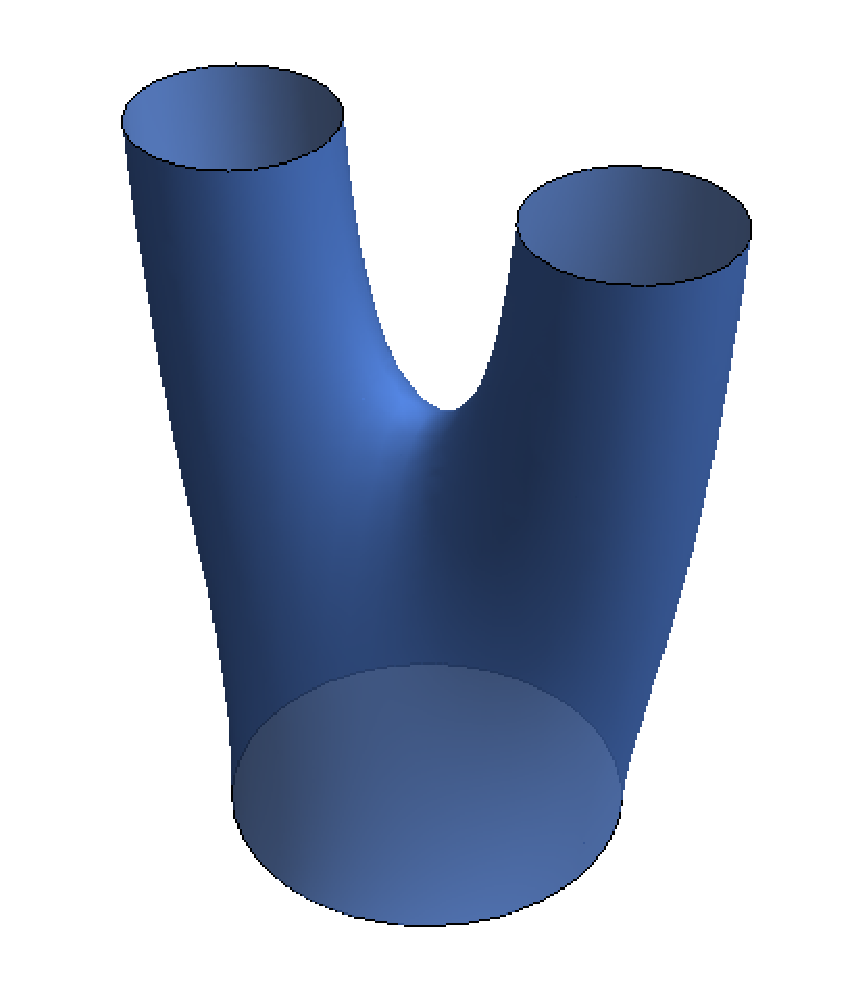
\includegraphics[
clip=true,
width=0.4\textwidth]
{trousers-3d-raw-rast.pdf}%trim=l b r t, clip=true,
\caption[]{The ``trousers'' spacetime with topology-change $S^1\leftrightarrow S^1\times S^1$.}
\label{fig:trousers-3d}
\end{figure}


The first work along these lines was carried out by Anderson and DeWitt~\cite{Anderson:1986ww}, who studied the quantum theory of a free massless scalar field on the topology-changing two-dimensional ``trousers'' spacetime, in which a circle splits into two (or vice-versa), viz. Figure~\ref{fig:trousers-3d}. This spacetime admits an almost everywhere Lorentzian metric, which is the flat Minkowski metric everywhere except at an isolated singular point --- the ``crotch singularity'' --- on the spatial hypersurface which separates the two spatial topologies. At the singular point the equations of motion degenerate and hence the rule by which to propagate solutions past it must be specified by hand. Expanding the scalar field in terms of modes on a spacelike hypersurface in one region (the ``in''-region) and choosing a particular ``shadow rule'' to propagate the modes past the topology-changing hypersurface into an ``out''-region, Anderson and DeWitt found that the expectation value of the ``out'' stress-energy tensor evaluated in the ``in''-vacuum has incurable (squared Dirac-delta) divergences on the lightcone of the singular point. They concluded that the trousers-type topology-change is dynamically forbidden. Manogue et al.~\cite{Copeland:1988tr} revisited the problem in a more careful analysis. They argued that the propagation rule of Anderson and DeWitt is unphysical because the Klein-Gordon product between two solutions obtained by propagating forward initial data past the topology-changing hypersurface is not conserved. Deriving a one-parameter family of propagation laws that conserve the inner product they arrived at the same conclusion, an infinite burst of energy emanating from the crotch singularity.
%a $\delta^2$-divergence on the lightcone of the singular point.

These results may at first be disappointing to those who hope that a quantum theory of gravity will incorporate topology-change. Of course, it could always be the case that the approximations made in such top-down calculations turn out to be wrong, but then again, without a bottom-up theory at hand, semi-classical calculations are one of the only tools we have to guide us. There are, however, good reasons why topology-change may still be physically viable even if the particular type of topology-change of the trousers spacetime is disallowed. The transition in the trousers belongs in a sense to a particularly singular class of topology-changes~\cite{Dowker:1997hj}, those in which the spacetime exhibits ``causal discontinuity'', which means (roughly) that the volume of the causal past or future of a point can change discontinuously as the point moves continuously around the manifold. The authors of~\cite{Louko:1995jw} found that causally discontinuous topology changing processes in $1+1$ dimensions are indeed suppressed in a sum-over-histories, while causally continuous ones are enhanced. Such observations lend some support to Sorkin's conjecture that infinite energy production occurs in a topology-changing spacetime\footnote{More precisely, a topological cobordism endowed with an almost everywhere Lorentzian metric, i.e. the first alternative of those mentioned above for turning topological cobordisms into geometries.} \emph{if and only if} it contains a causal discontinuity.

In this chapter we present the results of first efforts to address the problem within the framework of the SJ formalism. This approach works directly with propagators rather than with the field operator expanded in modes. The freedom in specifying a propagation law corresponds to a freedom in choosing retarded and advanced Green functions. Once these are specified, however, the formalism should select a quantum state without further input. In light of the previous paragraph, the expectation would be to \emph{confirm} previous findings in the trousers spacetime. The hope is to gain new insights by revisiting the problem from a new point of view, to understand the SJ framework in a more general setting, and to lay the foundation for semi-classical calculations in other topology-changing spacetimes.\\

%NEED TO MENTION http://xxx.lanl.gov/pdf/gr-qc/0004033v1.pdf !!!

%In order to address these questions, Anderson and de Witt introduced the so-called ``trousers'' spacetime, in which spatial sections are initial circle undergo a transition from a circle splits into two circles $S\rightarrow S\times S$.

%Let us put a flat Lorentzian metric in the trousers. This metric will have to degenerate (become Euclidean) in a neighbourhood of the crotch albeit an arbitrarily small one. This neighbourhood can be shrunk to a point, which we shall refer to as the crotch singularity. At this point, the metric degenerates and the equations of motion of matter fields become ill-defined. (An entirely equivalent point of views is to consider the crotch singularity as excised from the manifold).

%\noindent\textbf{Comment on use of language:}
%\textit{Propagators such as $G_R(x,y)$ are functions of two variables and hence to talk about their support or their functional form requires us to specify both arguments. However, it is customary to think and speak of propagators as functions of one variable by effectively fixing one argument. We will use the following conventions. When speaking of the support or functional form of a propagator, we will assume that the \emph{first} argument has been fixed and we refer to the function of a single variable whose one variable is the second argument. In this sense, the ``support of the retarded propagator'' is a past light-cone.}

\section{Quantum Fields in the trousers spacetime}\label{sec:qftintrousers}

%The general approach in this previous work has been to expand the field in the trunk and leg regions:
%\be
%\phi(x,t) =
%\begin{cases}
%\phi_T(x,t)\qquad&\text{for}\;t<0\\
%\phi_L(x,t)\qquad&\text{for}\;t>0
%\end{cases}
%\ee
%where $\phi_T$ and $\phi_L$ are solutions to the Klein-Gordon equation, and to impose Cauchy data for $\phi$ and $\pi=\dot\phi$ at $t=0^\pm$ which depends on the solution at $t=0^\mp$, thereby specifying a ``propagation rule'' for the field. The discontinuities in $\phi_{T,L}$ imply that the propagation rule must include delta-function singularities in $\pi_{T,L}$.

\begin{figure}[t!]
\centering
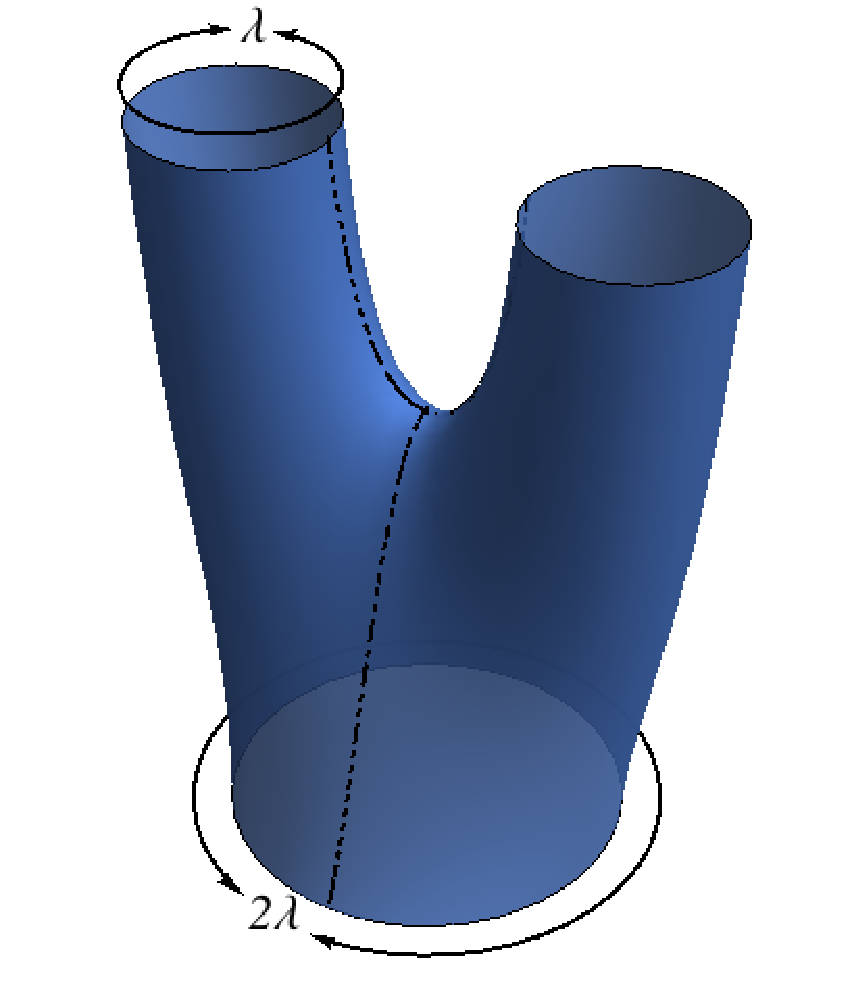
\includegraphics[
clip=true,
width=0.44\textwidth]
{trousers-3d-v3.pdf}%trim=l b r t, clip=true
\hspace{0.1\textwidth}
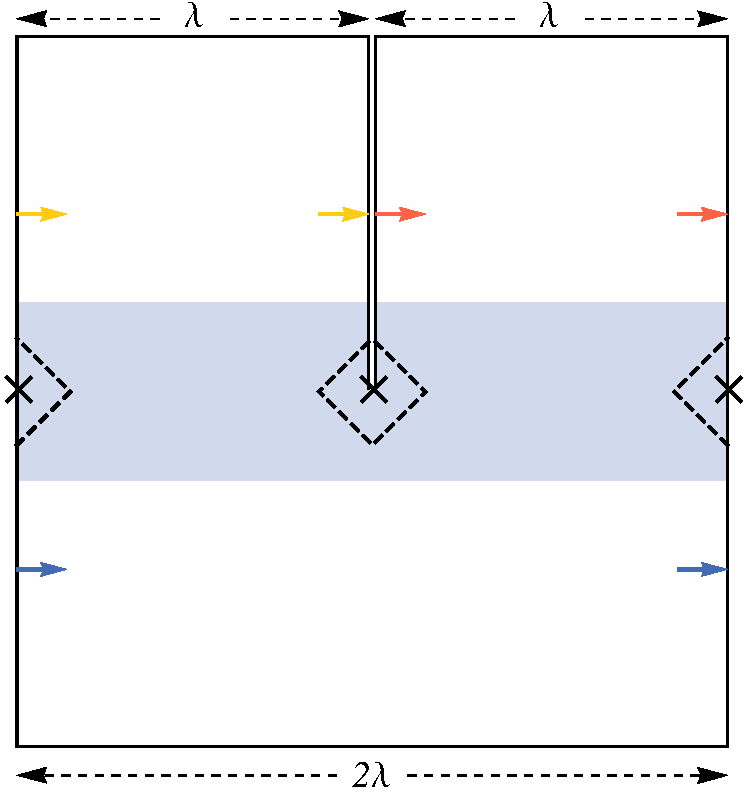
\includegraphics[
clip=true,
width=0.45\textwidth]
{trousers-flattened-labelled-v4.pdf}%trim=l b r t, clip=true
\caption[]{The trousers spacetime (left) and a two-dimensional representation of it (right) obtained by cutting and unwrapping the manifold. The coloured arrows indicate the respective identifications in the trunk (blue) and in the left and right legs (yellow and red). The crosses mark the location of the crotch singularity.}
\label{fig:trousers-flattened-raw}
\end{figure}

Keeping with tradition we hang the trousers upside down and use a coordinate chart in which $t=0$ separates the ``legs'' and the ``trunk''. The spatial coordinate $x$ lies in the range $[-\lambda,\lambda]$ and the crotch singularity lies at the origin: $x_c=(0,0)$. The coordinates in the trunk extend to coordinates in the left and right legs, i.e. we identify points $(x,0^+)$ in the legs with points $(x,0^-)$ in the trunk for $x\neq0$.  In the trunk, i.e. for $t<0$, we identify $x=-\lambda$ with $x=\lambda$. In the left leg, i.e. for $t>0$, we identify $x=-\lambda$ with $x=0^-$ and in the right leg we identify $x=\lambda$ with $x=0^+$. An illustration of the spacetime is shown in Figure~\ref{fig:trousers-flattened-raw}.\\

We will attempt to build the SJ state by identifying the positive eigenmodes of $i\Delta$ as we did in the analysis of the flat diamond. For this, we need the Pauli-Jordan function $\Delta=G_R-G_A$, and thus the retarded and advanced Green functions  in the trousers.

There are two ways in which the Green functions in the trousers differ from those in Minkowski space. The first is due solely to the topology of the spatial sections before and after the topology-change and is largely independent of the questions pertaining to topology-change. Consider the quantum field theory on a flat cylinder $S^1\times\,\mathbb R$ (no topology-change). The metric is Minkowskian and so the propagators are locally Green functions to the usual wave equation. However, the future/past lightcone of any point will wrap around the cylinder, which makes it inconsistent to use the naive solution $G^{\mathsf M_{}}_R(x,y)$ of two-dimensional Minkowski space $\mathsf M$, which is equal to $-\frac12$ in the causal past of $x$ (and zero everywhere else). At the first conjugate point $p_x$ to the past of $x$ (the point where the two past-directed null geodesics emanating at $x$ meet again), the naive Green function will take on the form $-\frac12(1-\theta(- u)\theta(- v))$ in light-cone coordinates centred at $p$. This produces a negative Dirac-delta type source $-\delta^{(2)}(x-p_x)$ in $\dAlembert_x G_R(x,y)$ and therefore the naive propagator will not be a Green function. However, it is not hard to obtain a modification that \emph{will} be a Green function, by simply taking $G^{\mathsf M_{}}_R(x,y)$ and adding to it a (multiple of) $G^{\mathsf M_{}}_R(p_x,y)$ for every conjugate point $p_x$ such that the divergences in the original function are cancelled.

%\begin{figure}[t!]
%\centering
%\includegraphics[
%clip=true,
%width=0.3\textwidth]
%{gret-on-cylinder.pdf}%trim=l b r t, clip=true,
%\caption{Naive retarded propagator on the cylinder.}
%\label{fig:pairofdiamonds}
%\end{figure}

The observations in the previous paragraph are not particular to the trousers --- they simply concern well-known facts of quantum field theory on the cylinder. 
%(although one encounters a similar phenomenon when we look at the retarded propagator near the crotch singularity). 
In order to isolate the features of the trousers spacetime that are most pertinent to the physics of topology-change, we can first restrict ourselves to a small enough section of the trousers containing the singularity such that no wrapping around occurs, e.g. $|t|\leq t_{max}$ for some $t_{max}<\frac\lambda4$ as shown in Figure~\ref{fig:trousers-flattened-raw} (the upper bound of $\frac\lambda4$ guarantees that the future lightcone of a point in the causal past of the singularity does have time to wrap around one of the legs). In fact, it will be most convenient to restrict our analysis to a small causally convex neighbourhood around the singularity. Hence consider two points, one in the left and one in the right leg, both in the chronological future of the singularity: $x_{L}^\pm=(t_0,\pm\epsilon)$. Take the intersection of the union of their causal pasts with the causal future of a point in the trunk, $x_{T}=(-t_0,0)$, which lies in the chronological past of the singularity. In the limit that the two points $x^\pm_L$ are chosen to lie arbitrarily close to $x=0$ this region of spacetime will consist of the two diamonds drawn with dashed lines in Figure~\ref{fig:trousers-flattened-raw}. We refer to this spacetime as the \emph{pair of diamonds}. Figure~\ref{fig:pairofdiamonds} gives a more detailed depiction of the pair of diamonds, with the topological identifications inherited from the trousers. This spacetime has the same essential causal properties as the topology-changing trousers.

\begin{figure}[t!]
\centering
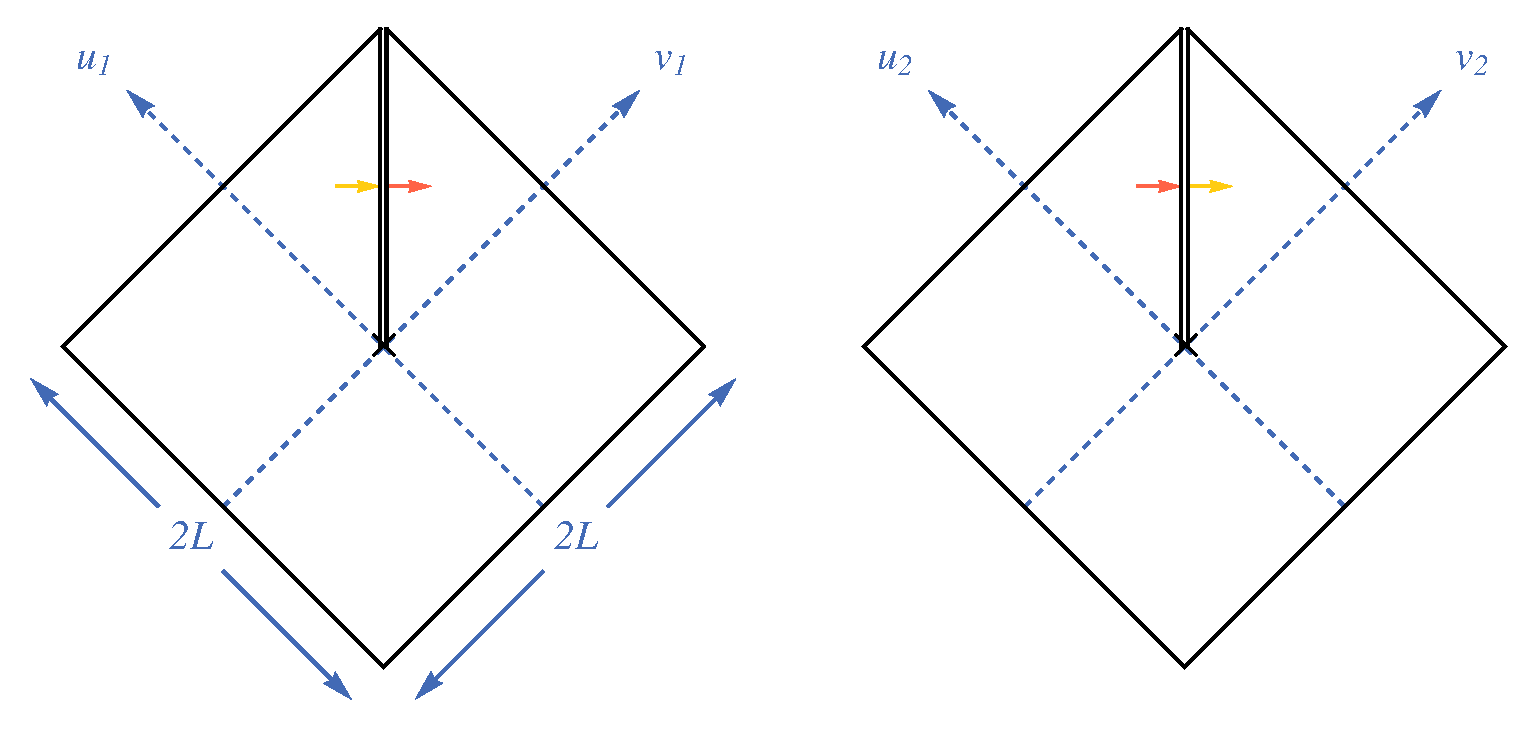
\includegraphics[
clip=true,
width=\textwidth]
{pairofdiamonds-v2.pdf}%trim=l b r t, clip=true,
\caption[]{The pair of diamonds in more detail. The coloured arrows indicate the topological identifications inherited from the trousers (Figure~\ref{fig:trousers-flattened-raw}).}
\label{fig:pairofdiamonds}
\end{figure}

\section{The pair of diamonds}

In order to discuss the pair of diamonds and functions on it we need to construct a coordinate chart that covers the spacetime. When we depict the two diamonds next to each other, the left diamond is meant to corresponds to the diamond seen in the centre of the trousers (Figure \ref{fig:trousers-flattened-raw}) and the right diamond is made up of the two halves at the sides of the trousers. We will refer to the left and right diamonds as diamond $1$ (symbol $D_1$) and diamond $2$ (symbol $D_2$). Hence the upper left and right corners in diamond $1$ respectively belong to the left and right legs, whereas the upper left and right corners in diamond $2$ respectively belong to the right and left legs.
Now define two identical coordinate systems with subscripts $1$ and $2$ on $D_1$ and $D_2$. We will use both Cartesian and light-cone coordinates below and we shall label them in the obvious manner, e.g. $(u_1,v_1)$ and $(u_2,v_2)$ denote light-cone coordinates on $D_1$ and $D_2$ respectively. The relationship between the trousers coordinates (without subscript) defined above and the coordinates on the two diamonds are as follows. On diamond $1$ the coordinate systems agree since their origin is the same. So
%%%\be
%%%\begin{aligned}
%%%t_1&=t\\
%%%x_1&=x
%%%\end{aligned}
%%%\iff
%%%\begin{aligned}
%%%u_1&=u\\
%%%v_1&=v
%%%\end{aligned}
%%%\ee
$t_1=t,x_1=x,u_1=u$ and $v_1=v$. On diamond $2$, the left side comes from the right edge of the trousers and the right side comes from the left edge of the trousers,  so the relations between the coordinates on $D_2$ and those in the trousers are
\be
\begin{aligned}
t_2 &= t\\
x_2&=x-\lambda\quad\text{for}\;x>0\\
x_2&=x+\lambda\quad\text{for}\;x<0
\end{aligned}
\quad\iff\quad
\begin{aligned}
\left.
\begin{aligned}
u_2&=u+\lambda/\sqrt2\\
v_2&=v-\lambda/\sqrt2
\end{aligned}
\quad\right\}
\quad\text{for}\;x>0\hphantom{.}\\
\left.
\begin{aligned}
u_2&=u-\lambda/\sqrt2\\
v_2&=v+\lambda/\sqrt2
\end{aligned}
\quad\right\}
\quad\text{for}\;x<0.
\end{aligned}
\ee
The coordinate ranges are $u_i,v_i\in[-L,L]$ for $i=1,2$ where $L<\lambda$ sets the length scale of the diamonds. In both coordinate systems the crotch singularity is at the origin of coordinates. For $0<t_1,t_2<\sqrt{2}L$ we identify $x_1=(v_1-u_1)/\sqrt{2}=0^-$ with $x_2=(v_2-u_2)/\sqrt{2}=0^+$ and vice versa. This gives us a complete chart on the pair of diamonds. Of course the two coordinate systems do not correspond to a split into left and right legs in the embedding trousers manifold: for example, both the top left part of $D_1$ (i.e. $u_1>v_1>0$) and the top right part of $D_2$ (i.e. $v_2>u_2>0$) belong to the left leg of the trousers.

To make expressions simpler we will typically use coordinates without subscript to describe functions on the pair of diamonds, and we will use an indicator function to restrict support onto subregions.
Hence for a subregion $R$ we write $R(x)$ to denote the function which is equal to $1$ when $x\in R$ and zero otherwise (this is commonly also seen as $\mathbf 1_R(x)$). For instance, $f(x)=e^{iku}$ is shorthand for $f(x)=e^{iku_1}D_1(x)+e^{iku_2}D_2(x)$, and $g(x)=e^{iku}D_1(x)$ is shorthand for the function that is equal to $e^{iku_1}$ in diamond $1$ and zero in diamond $2$. (This function should not be confused with the Boolean function $\chi$ defined earlier, which we will also use below and which maps propositions to $\{0,1\}$: $\chi(A)=1$ if $A$ is true and $\chi(A)=0$ if $A$ is false.) Note that, in these conventions, $f(u)D_2(x)$ is \emph{not} equal to $f(u)$ on $D_2$: it is equal to $f(u_2)=f(u-\lambda/\sqrt2)$.

Each diamond splits naturally into five regions:
\begin{enumerate}
\item Bottom: the causal past of the singularity
\item Centre Left: the region spacelike to and to the left of the singularity
\item Centre Right: the region spacelike to and to the right of the singularity
\item Top Left: the left part of the causal future of the singularity
\item Top Right: the right part of the causal future of the singularity
\end{enumerate}
These regions, along with some additional ones that will be used below, are defined more comprehensively for diamonds $1$ and $2$ on Table~\ref{tab:pod-regions}. As described above, we will also use the symbols defined here as indicator functions, e.g. $\Bone(x)$ is one if $x$ is in the bottom of diamond $1$ and zero otherwise. 


%VERSION WITH SYMBOLS
\begin{table}[t!]
\begin{center}
%
\begin{tabular}{llc}
  \textbf{Symbol} &\textbf{Name}&\textbf{Definition}\\
\toprule
$\TLone$&Top Left 1& $u_1>v_1>0$\\
\midrule
$\TRone$&Top Right 1& $v_1>u_1>0$\\
\midrule
$\MLone$&Middle Left 1& $v_1<0 \textrm{ and } u_1>0$\\
\midrule
$\MRone$&Middle Right 1& $v_1>0 \textrm{ and } u_1<0$\\
\midrule
$\Bone$&Bottom 1& $v_1<0 \textrm{ and } u_1<0$\\
\midrule
$\ULDone$&Upper Left Diagonal 1 & $\MLone\cup \TLone\cup \TRtwo$\\
\midrule
$\URDone$&Upper Right Diagonal 1 & $\MRone \cup \TRone\cup \TLtwo$\\
\midrule
$\LLDone$&Lower Left Diagonal 1& $\Bone\cup \MLone$\\
\midrule
$\LRDone$&Lower Right Diagonal 1 & $\Bone \cup \MRone$\\
\midrule
$\LL$	  &Left Leg				& $\TLone\cup \TRtwo$\\
\midrule
$\RL$	  &Right Leg & $\TRone\cup \TLtwo$\\
\midrule
$\POD$	  &Pair of Diamonds & $\cup$ all of the above\\
\bottomrule
\end{tabular}
%
\end{center}
\caption[]{Some subregions of the pair of diamonds and their labels. All regions except the last two are defined with respect to $D_1$ --- for these there are analogous regions defined with respect to $D_2$. Note that the upper left and right diagonal regions as well as the left and right leg regions extend over both diamonds (as evident in their symbols).}
\label{tab:pod-regions}
\end{table}

%VERSION WITH LETTERS:
\iffalse
\begin{table}
\begin{center}
%
\begin{tabular}{llc}
  \textbf{Abbreviation} &\textbf{Name}&\textbf{Definition}\\
\toprule
$TL_1$&Top Left 1& $u_1>v_1>0$\\
\midrule
$TR_1$&Top Right 1& $v_1>u_1>0$\\
\midrule
$L_1$&Middle Left 1& $v_1<0 \textrm{ and } u_1>0$\\
\midrule
$R_1$&Middle Right 1& $v_1>0 \textrm{ and } u_1<0$\\
\midrule
$B_1$&Bottom 1& $v_1<0 \textrm{ and } u_1<0$\\
\midrule
$ULD_1$&Upper Left Diagonal 1 & $L_1\cup TL_1\cup TR_2$\\
\midrule
$URD_1$&Upper Right Diagonal 1 & $R_1\cup TR_1\cup TL_2$\\
\midrule
$LLD_1$&Lower Left Diagonal 1& $B_1\cup L_1$\\
\midrule
$LRD_1$&Lower Right Diagonal 1 & $B_1 \cup R_1$\\
\bottomrule
\end{tabular}
%
\end{center}
\caption[.]{
Regions and their labels as defined for $D_1$. Analogous definitions hold for regions associated with $D_2$. Note that ${\TLDone}$ and $URD_1$ extend over both diamonds.
}
\label{tab:pod-regions}
\end{table}
\fi

Whether one considers the crotch as excised from the manifold or as a point that is present but at which the metric degenerates, the wave equation invariably loses its meaning there. For field modes this requires the specification of a propagation law, and in particular a rule for how a solution before/after the topology-change is to be propagated past the singularity. In terms of Green functions we are faced with a choice of what the retarded and advanced propagators look like near the singularity. This leads to a departure of the usual story in a number of ways. Not only is there a need to motivate any specific functional form of the retarded and advanced propagators, but the symmetry between the two is not forced upon us anymore.%, as it is already apparent from the clear breakdown of time symmetry as the topology-change occurs.

\section{Propagators in the trousers}
% divergence theorem with null boundaries
% http://www.ictp-saifr.org/schoolgr/Lecture0Friedman.pdf
%http://en.wikipedia.org/wiki/Laplace_operator
%http://mathoverflow.net/questions/132879/hodge-decomposition-in-minkowski-space

Since the d'Alembertian degenerates at the singularity, it is unclear what is meant by a propagator as a Green function to the equations of motion. For pairs of points whose causal interval $[x,y]$ does not contain the singularity, the retarded propagator should take its usual $\mathsf M$-form $G_R(x,y)=-\frac12\chi(x\succ y)$, since $G_R$ satisfies the equations of motion and retarded boundary conditions everywhere in $[x,y]$. But what happens when the interval $[x,y]$ contains the singularity, i.e. when the topology-change ``registers'' in the evolution between two spacetime points? The most naive ansatz would be to set $G_R(x,y)=-\frac12\chi(x\succ y)$ for \emph{all} pairs of points in the trousers, leaving the evolution law unchanged. This is illustrated in Figure~\ref{fig:gret-on-pod-false}. This however leads to inconsistencies, as a more careful analysis in the following paragraphs shows.
\begin{figure}[t]
\centering
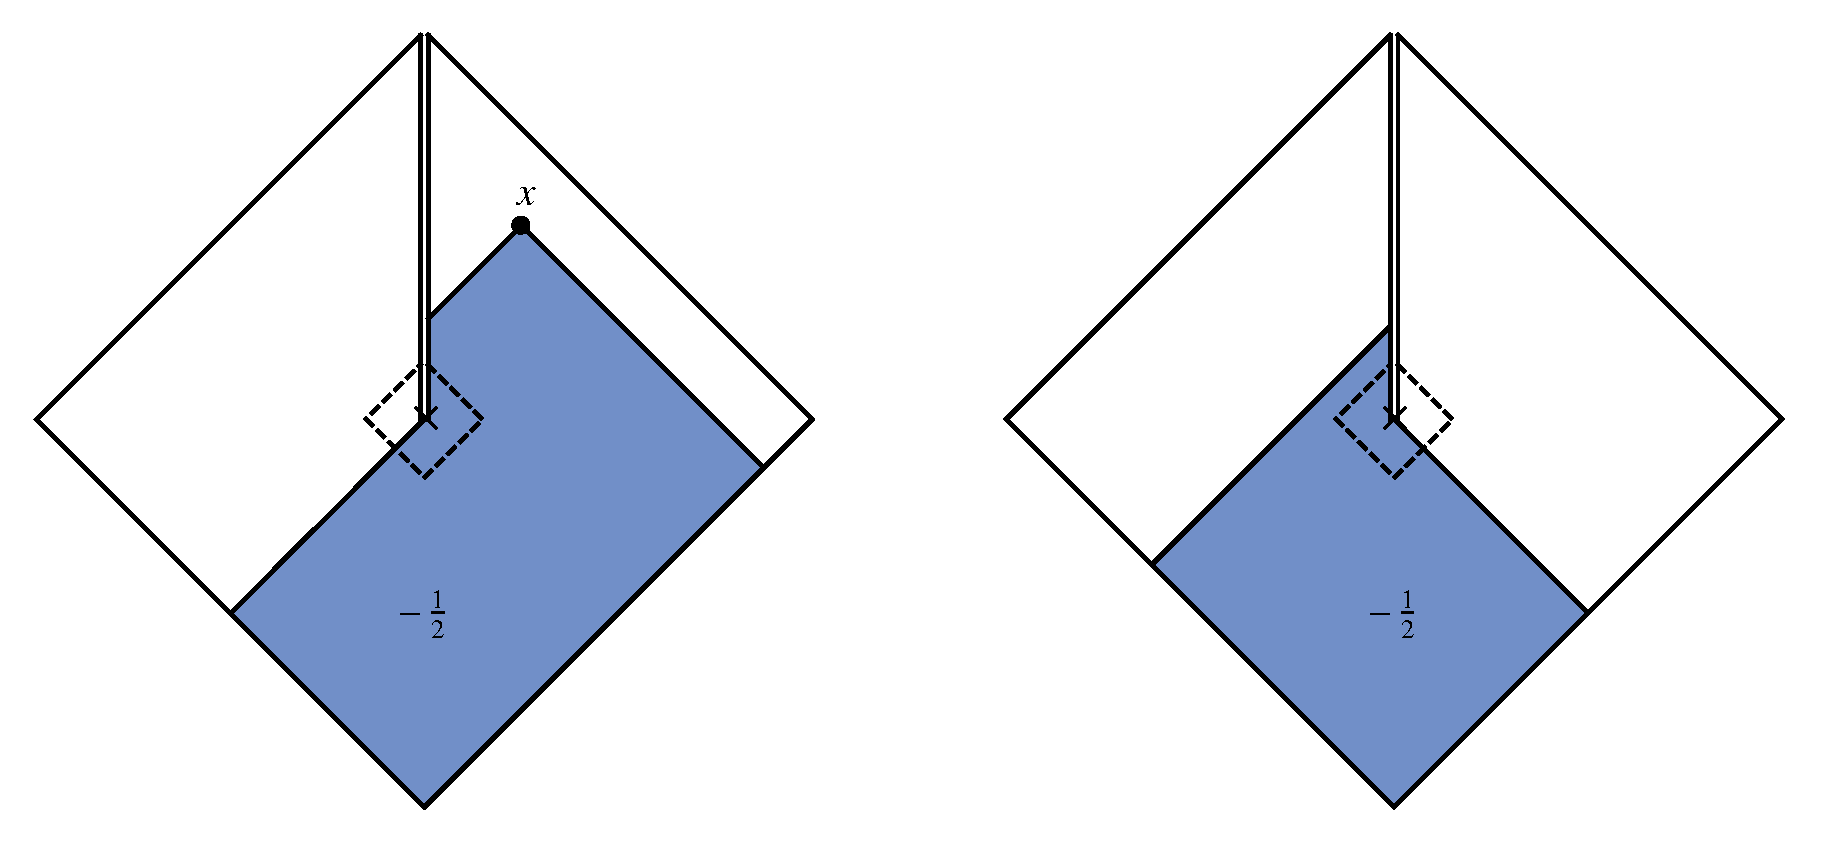
\includegraphics[
clip=true,
width=\textwidth]
{gret-on-pod-false.pdf}%trim=l b r t, clip=true,
\caption[]{A naive ansatz for the retarded propagator $G_R(x,y)=-\frac12\chi(x\succ y)$ in the trousers, drawn as a function of $y$ for fixed $x\succ x_c$ represented by the black dot. The function is equal to $-\frac12$ in the shaded region and zero everywhere else. The dashed contour corresponds to the boundary of a causal diamond centred on the singularity.}
\label{fig:gret-on-pod-false}
\end{figure}

\subsection{Integral form of Green's equation}

We start with the following observation. In any neighbourhood $D\subset\mathsf M$ of ordinary (two-dimensional) Minkowski space the operator $\dAlembert$ is well-defined and we call $G(x,y)$ a Green function if it satisfies $\dAlembert_x G(x,y) = \dAlembert_y G(x,y)= \delta^{(d)}(x,y)$ for all $x,y\in D$, denoting by $\dAlembert_x$ the d'Alembertian with respect to argument $x$. Let us assume for now that $D$ is a causal diamond. We will work in light-cone coordinates $y^\mu=(u,v)$ and we define $G_x(y):=G(x,y)$, by which we mean that $G_x(y)$ is to be thought of as a function of a single argument $y$ for fixed $x$. Then Green's equation on one hand implies
\be
\int_D dudv \dAlembert G_x(u,v)=\int_D \delta(u-u_x)\delta(v-v_x)dudv = D(x),
\ee
recalling that $D(x)$ is the indicator function equal to $1$ if $x\in D$ and zero otherwise. On the other hand, using Green's theorem for a right-handed Cartesian coordiante system $(u,v)$:
\be
\int_D \left(\partial_v M -\partial_u L\right)dudv = \oint_{\partial D} L dv + M du
\ee
with $M =-\partial_u G_x$ and $L=\partial_v G_x$ we find
\bea
\int_D dudv \dAlembert G_x(u,v)
%&=\int_D dudv\, (-2)\partial_u\partial_vG_x(u,v)\\
&=\oint_{\partial D}\left(\partial_v G_x(u,v) dv -\partial_u G_x(u,v) du \right)
\eea
%\bea
%\int_Vd\mu_V\,\dAlembert G
%&=\int_V\sqrt{-g}\,d^dx\,\nabla^\mu\nabla_\mu G(x,y)\\
%&=\int_{\partial V}\epsilon \sqrt{|h|}d^{d-1}x n^\mu \partial_\mu G(x,y)
%\eea
where the null boundary $\partial D$ of the causal diamond is to be traversed in anti-clockwise fashion.\footnote{
This formula of course only holds in flat space. The direction of the contour integral on the right hand side is determined by the handedness of the coordinate system on $D$. %Usually the theorem is stated for right-handed coordinates $(x,t)$, i.e. $x$ increasing to the right and $t$ increasing upward. For such coordinates the direction of the contour-integral is indeed counter-clockwise. Lightcone coordinates $(u,v)$ have the same handedness since they are obtained by a $45^\circ$ rotation from $(x,t)$. 
The general (curved spacetime) formula afforded by Stokes' theorem is more subtle in the Lorentzian setting (especially in the presence of null boundaries) due to the indefinite signature of the metric. See~\cite{sorkin:stokes,garcia1998divergence} for details.
%See Appendix~\ref{app:stokes} for a more detailed discussion.
}
Hence for any causal diamond $D$ in $\mathsf M$, a Green function will satisfy
\be
\label{eq:alternativegreen}
\oint_{\partial D}\left[\partial_v G_x(u,v) dv -\partial_u G_x(u,v) du \right] = D(x).
\ee
This relation is valid for both arguments and applies to the retarded and advanced Green functions. For instance, it can easily be verified for $G_R(u,v)=-\frac12 \theta(u)\theta(v)$. Let us denote the integral in~\eqref{eq:alternativegreen} by $\mathfrak B^{D}_y G(x,y)$. Then we can write an integral version of Green's equation as
\be
\mathfrak B ^D_y\left[G_R(x,y)\right]=D(x).
\label{eq:contour-op}
\ee


\subsection{The field equations near the singularity}
We turn to the pair of diamonds. For ease of notation we denote by $\mathfrak B_y\left[G(x,y)\right]$ (with no superscript) the contour integral for which $D$ is a small causally convex neighbourhood $D$ whose interior contains the singularity $x_c$ but \emph{not} $x$. Similarly, $\mathfrak B_x\left[G(x,y)\right]$ is the contour integral around a contour whose interior contains $x_c$ but not $y$. In order for $G(x,y)$ to ``satisfy Green's equation'' at the singularity we then need~\eqref{eq:alternativegreen}
\bea
\label{eq:alternativegreen2}
\mathfrak B_y\left[G_R(x,y)\right] =\mathfrak B_x\left[G_R(x,y)\right] = 0.
\eea
Now it can easily be seen that this will \emph{not} be the case for the naive ansatz $G_R(x,y)=-\frac12\chi(x\succ y)$. As illustrated in Figure~\ref{fig:gret-on-pod-false}, we obtain $+1$ instead of zero on the right hand sides of~\eqref{eq:alternativegreen2}. There are two ways to see this. One is to note that the only contributions to the contour integral come from the places where the propagator changes between $-\frac12$ and $0$, and at both places the derivative in $\mathfrak B _y\left[G_R(x,y)\right]$ picks up $+\frac12$. The other way is to see that in effect the ``shadow'' of the retarded propagator doubles up below the singularity, which corresponds to an extra Dirac-delta type term centered at the singularity in Green's equation. The same can be observed for $G_A(x,y)$, whose support ``streams out'' into both legs when $x\prec x_c$. Therefore $\Delta=G_R-G_A$ constructed from the naive propagators will not be a solution to the equations of motion near the crotch in the sense that $\mathfrak B_y\left[\Delta(x,y)\right]\neq 0$ and $\mathfrak B_x\left[\Delta(x,y)\right]\neq 0$.

These observations are reminiscent of the singularities in $G^{\mathsf M_{}}_R(x,y)$ at conjugate points on the cylinder: the crotch singularity appears as a spurious source in the equations of motion. On the cylinder a physically satisfying propagator can be constructed by adding to the naive propagator appropriate scalar multiples of itself centred at the conjugate points. We shall follow a similar line of thought in order to construct viable propagators in the trousers. The situation is not as simple, however. To begin with, there is no time-reversal symmetry in the trousers spacetime and hence the usual a priori assumption of perfect symmetry between retarded and advanced propagators seems unwarranted. Furthermore, in the globally hyperbolic case it is true that $\dAlembert_x G_R(x,y)=\delta^{(2)}(x-y)\iff\dAlembert_y G_R(x,y)=\delta^{(2)}(x-y)$ provided the boundary conditions are satisfied, while the analog relation
\be
\mathfrak B_y\left[G_R(x,y)\right]=0\iff\mathfrak B_x\left[G_R(x,y)\right]=0\label{eq:twoeoms}
\ee
does not obviously obtain without global hyperbolicity. This is closely related to the following fact: if $x\in\Bone$, $y\in\TLone$ and $y'\in\TRone$, then it is a priori not required that $G_R(x,y)$ take the same value for $(x,y)$ as it does for $(x,y')$ --- different such values implying different ``strengths of propagation'' into the left and right legs --- so there is a potentially richer class of propagators corresponding to different physics. To construct a general family of propagators for the trousers, a more careful review is in order.\\

\subsection{A one-parameter family of propagators}
Recall that in the usual construction of the quantum theory, the primary role of the retarded and advanced propagators is their appearance in the Pauli-Jordan function $\Delta = G_R - G_A$. The latter enforces the causality structure of the theory, which is imposed through the commutation relations $[\phi(x),\phi(y)]=i\Delta(x,y)$ (or their equal-time version, the canonical commutation relations). In order to act as a commutator of fields $i\Delta$ should thus be antisymmetric. Antisymmetry also guarantees that $i\Delta$ is a Hermitian integral kernel, which is essential in the construction of the SJ state. It is therefore reasonable to require that the propagators should \emph{at least} be consistent with $\Delta$ being antisymmetric and a solution to the field equations in both arguments in the sense of~\eqref{eq:alternativegreen}:
\be
\mathfrak B ^D_y\left[\Delta(x,y)\right]=\mathfrak B ^D_x\left[\Delta(x,y)\right]=0.
\ee
So let us define $G_R$ and $G_A$ to be the retarded and advanced parts of the commutator
\bea
G_R(x,y)&=\chi(x\succ y)\Delta(x,y)\\
G_A(x,y)&=-\chi(y\succ x)\Delta(x,y).\label{eq:newdefofprop}
\eea
and impose the conditions $\Delta=-\Delta^T$ and $\mathfrak B\Delta=0$ in both arguments. By consequence of~\eqref{eq:newdefofprop}, $G_R$ and $G_A$ as well as any one $G$ and its transpose $G^T$, clearly have disjoint supports. This together with the antisymmetry of $\Delta$ implies
\be
G_R(x,y)=G_A(y,x).\label{eq:podpropcond1}
\ee
We see that the antisymmetry of $\Delta$ indeed \emph{implies} the symmetry between advanced and retarded propagators. The equations of motion require that
\bea
\mathfrak B_x\Delta(x,y)=\mathfrak B_x G_R(x,y) - \mathfrak B_x G_A(x,y) &=0\\
\mathfrak B_y\Delta(x,y)=\mathfrak B_y G_R(x,y) - \mathfrak B_y G_A(x,y) &=0.
\eea
Together with~\eqref{eq:podpropcond1} this implies that if any one propagator is a solution to Green's equation in one of its arguments, then it, as well as its counterpart, must be solutions in both arguments.

\begin{figure}[t]
\centering
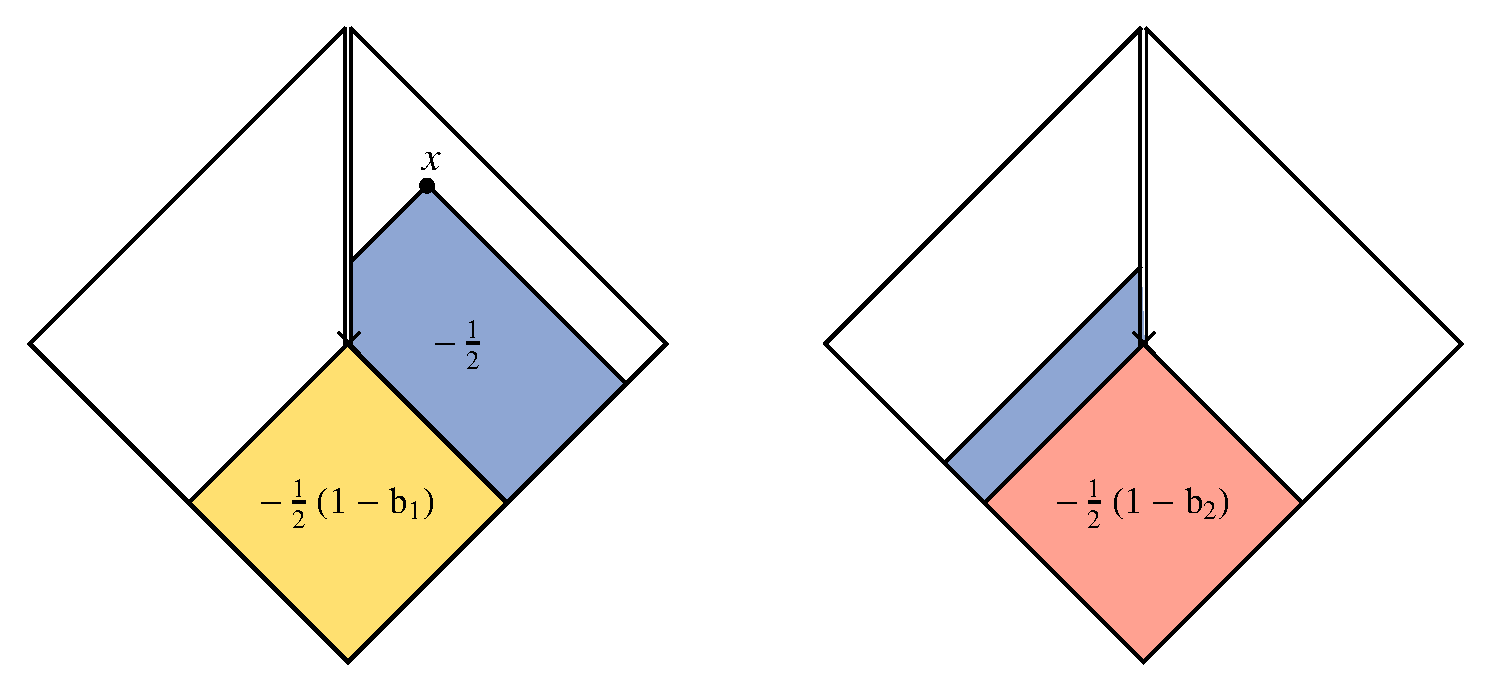
\includegraphics[
clip=true,
width=1.0\textwidth]
{gret-pod-modified.pdf}%trim=l b r t, clip=true,
\caption[]{The modified propagator $G_R(x,y)=G_A(y,x)$ for fixed $x$ in $\protect\TRone$. In order for the integral version of Green's equation to vanish for a small contour around the singularity, we need $b_1+b_2=1$.}
\label{fig:gret-on-pod-bs}
\end{figure}

So let us assume that the latter holds. Consider the retarded propagator $G_R(x,y)$. For $x\in\LL$ the spurious source at the crotch singularity that appears when $y\in\Bone$ or $y\in\Btwo$ can be cancelled by subtracting a linear combination of constant functions from the usual $-\frac12\chi(x\succ y)$. Whence for $x\in\LL$ we may propose a propagator of the form
\be
\left.G_R(x,y)\right|_{x\in\LL}=-\frac12\left[\chi(y\prec x)-a_1\Bone(y)-a_2\Btwo(y)\right].
\ee
In order for the contour integral $\mathfrak B_y G_R(x,y)=0$ to vanish we find that we must set $a_1+a_2=1$. Similarly, for $x\in\RL$ we can achieve $\mathfrak B_y G_R(x,y)=0$ if we set the propagator to
\be
\left.G_R(x,y)\right|_{x\in\RL}=-\frac12\left[\chi(y\prec x)-b_1\Bone(y)-b_2\Btwo(y)\right].\label{eq:gret-on-pod-bs}
\ee
with $b_1+b_2=1$. See Figure~\ref{fig:gret-on-pod-bs} for a visualisation of propagator~\eqref{eq:gret-on-pod-bs}. This leaves us with a two-parameter family of retarded propagators in the trousers (parameters $a:=a_1=1-a_2$ and $b:=b_1=1-b_2$). However, from $\mathfrak B_x G_R(x,y)=0$ we now obtain two additional constraints: to satisfy the equation for $y\in\Bone$, we need $a_1+b_1=1$, and to satisfy it for $y\in\Btwo$, we need $a_2+b_2=1$. This illustrates the decoupling of the equations of motion with respect to the first and second arguments referred to above~\eqref{eq:twoeoms}: none of the two equations (supplemented with boundary conditions) specifies a unique solution (as it would in a globally hyperbolic spacetime) --- instead, the two equations impose independent constraints on the solution.

We are thus left with a one-parameter family of retarded and advanced propagators $G_{R,p}(x,y)=G_{A,p}(y,x)$ parametrised by $p:=a_1=b_2=1-a_2=1-b_1$. For completeness we also show the propagator $G_A(x,y)=G_R(y,x)$ for fixed $x$ in the past of the crotch in Figure~\ref{fig:gadv-on-pod-ps}. 

The case $p=\frac12$ corresponds to the symmetric case in which the added negative source propagates with equal strength into and out of the two legs (see Figures~\ref{fig:gret-on-pod-bs} and~\ref{fig:gadv-on-pod-ps}, respectively). The cases $p=0$ and $p=1$ correspond to the two opposite extremes in which the source either only propagates into (and out of) the left leg, or into (and out of) the right leg. It is worth emphasising that these additional sources in the retarded and advanced propagators do \emph{not} in themselves yet constitute a ``burst in energy''. They do of course influence the propagation of the field past the singularity, and the effect of the added sources on the propagation might well translate into divergences in the stress-energy tensor. However, in order reach such conclusions, one first has to obtain the quantum state (through the Wightman function, or, equivalently, a complete set of positive frequency modes) and compute the expectation value of physical observables therein.

\begin{figure}[t]
\centering
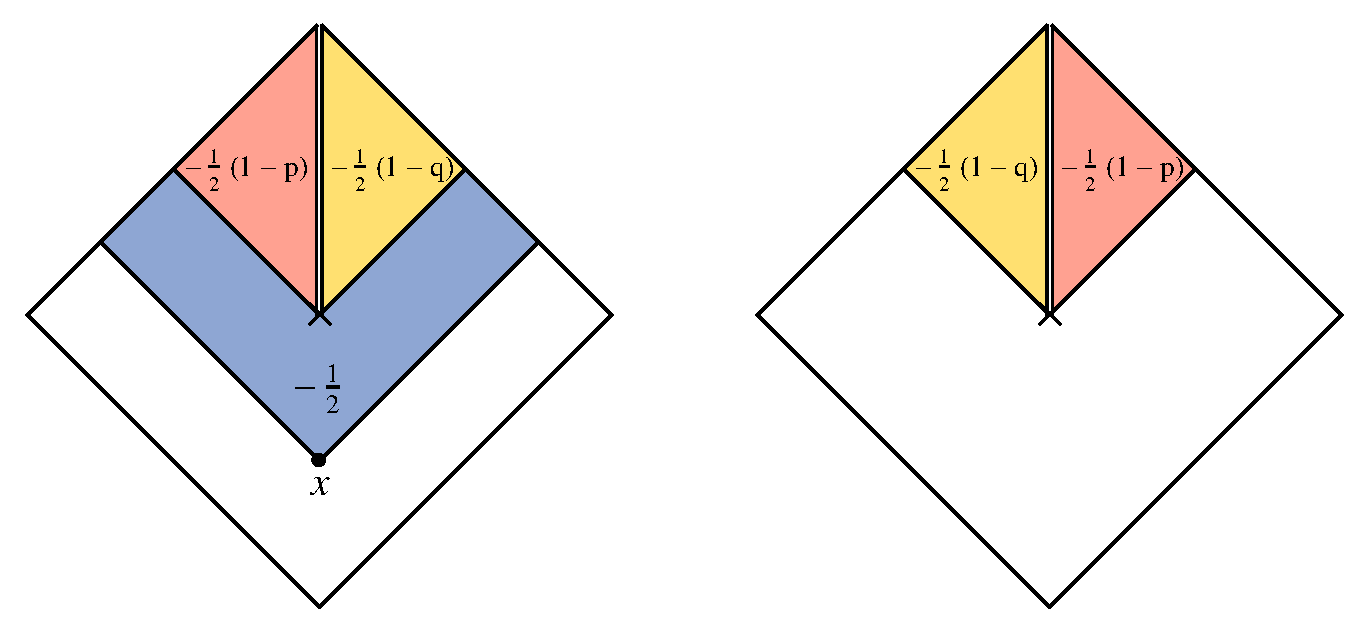
\includegraphics[
clip=true,
width=1.0\textwidth]
{gadv-pod-modified.pdf}%trim=l b r t, clip=true,
\caption[]{The modified propagator $G_{A,p}(x,y)=G_{R,p}(y,x)$ for fixed $x$ in $\protect\Bone$. Here $q=1-p$.}
\label{fig:gadv-on-pod-ps}
\end{figure}


\section{Propagation of plane waves past the singularity}\label{sec:proppastsing}
What type of propagation law do the propagators defined in the previous section entail? To understand this let us consider modes in the trunk and propagate them forward past the singularity using the retarded propagator. This can be done explicitly using Stokes' theorem (or its special case known as Green's second identity). We recall the usual evolution procedure of initial data with a retarded propagator. Given a solution $f(x)$ of the field equations (and its derivative) on a spacelike hypersurface $\Sigma$ and a retarded Green function $G_R(x,y)$ of the wave equation, one obtains the forward-propagated solution at a point $x$ in the future domain of dependence of the hypersurface $D^+(\Sigma)$ via an integral involving $G_R(x,y)$ and $f(x)$ over the section $J^-(x)\cap\Sigma$ of the hypersurface (where $J^-(x)=\left\{y:y\prec x\right\}$):
\be
f(x) = \int_{J^-(x)\cap\Sigma} d\Sigma_y^\mu\left[f(y)\nabla^y_\mu G_R(x,y)-G_R(x,y)\nabla^y_\mu f(y)\right].\label{eq:forwardprop}
\ee
Now we know that for $G_R(x,y)=-\frac12\chi(x\succ y)$, plane waves $u_k(x)=e^{-iku}$ (or $v_k(x)=e^{-ikv}$) will propagate forward to themselves, i.e. if $x$ is in the future domain of dependence of a hypersurface on which the solution is a plane wave, then~\eqref{eq:forwardprop} will yield the same plane wave evaluated at $x$.

Consider now the evolution generated by the modified retarded propagator $G_{R,p}$ on the pair of diamonds. Intuitively it is clear that a right-moving (left-moving) plane wave will just propagate freely along a diagonal $u=const.$ ($v=const.$) line and it will be oblivious to the singularity until it enters its future lightcone. What happens there? To find out, let us denote by $u^{\mathsf 1}_k(x)$ initial data corresponding to a right-moving plane wave in the trunk region of diamond 1 which is zero in the trunk region of diamond 2, i.e. $u^{\mathsf 1}_k(x)=e^{-iku}\NFone(x)$. Using the evolution equation we find that the wave evolves to $e^{-iku}-p$ for $x\in\LL$ (i.e. in the left leg) and to $+p$ for $x\in\RL$ (i.e. in the right leg). The constant terms in fact appear in the form $p e^{-iku_c}$ but since and $u_c=0$ in our coordinates this reduces to $p$. The complete forward-propagated solutions for initial data corresponding to right- and left-movers in the trunk regions of diamonds 1 and 2 are given by:
\bea
\label{eq:u1u2}
u^1_k(x)&=e^{-iku}\FPUone(x) + p\left[\LL(x)-\RL(x)\right]\\
u^2_k(x)&=e^{-iku}\FPUtwo(x) + p\left[\RL(x)-\LL(x)\right]\\
\eea
and
\bea
v^1_k(x)&=e^{-ikv}\FPVone(x) + (1-p)\left[\LL(x)-\RL(x)\right]\\
v^2_k(x)&=e^{-ikv}\FPVtwo(x) + (1-p)\left[\LL(x)-\RL(x)\right].
\eea
To find the evolution of plane waves in the \emph{whole} trunk it suffices to take linear combinations of the above modes. Due to the periodicity on the actual trousers, the modes on the pair of diamonds corresponding to the natural ``right-moving plane waves in the trunk'' with periodic boundary conditions take the form $u_k^1(x)+(-1)^n u_k^2(x)$ with $k=\sqrt{2}n\pi/\lambda$ in our conventions (the factor of $\sqrt2$ here comes from the factor of $\sqrt2$ in our definition of the lightcone coordinates). For even $n$, the constant terms in~\eqref{eq:u1u2} cancel. For odd $n$, they add up, leading to opposite constant terms $\pm 2p$ in the causal futures of the singularity pertaining to the left/right legs. Similar statements apply to left-moving incoming modes. Interestingly, this corresponds precisely to the one-parameter family of propagation laws found in~\cite{Copeland:1988tr}, which the authors arrived at by demanding the conservation of inner products under the evolution past the singularity (our parameter $p$ is related to their parameter $A$ via $p=\frac12(1+A)$).
 
\section{Eigenmodes of the Pauli-Jordan function}
The one-parameter family of propagators derived in the previous section provides us with a one-parameter family of Pauli-Jordan functions $\Delta_p = G_{R,p} - G_{A,p}$. It is not very illuminating to write down its functional form; for an example in pictorial form see Figure~\ref{fig:pj-on-pod}. When both arguments are outside the domain of influence of the crotch, $\Delta$ takes on its usual Minkowski form. Our aim is now to find the positive eigenfunctions of $i\Delta$ that satisfy $i\Delta(f) = \lambda f$ for $\lambda>0$.

\begin{figure}[t!]
\centering
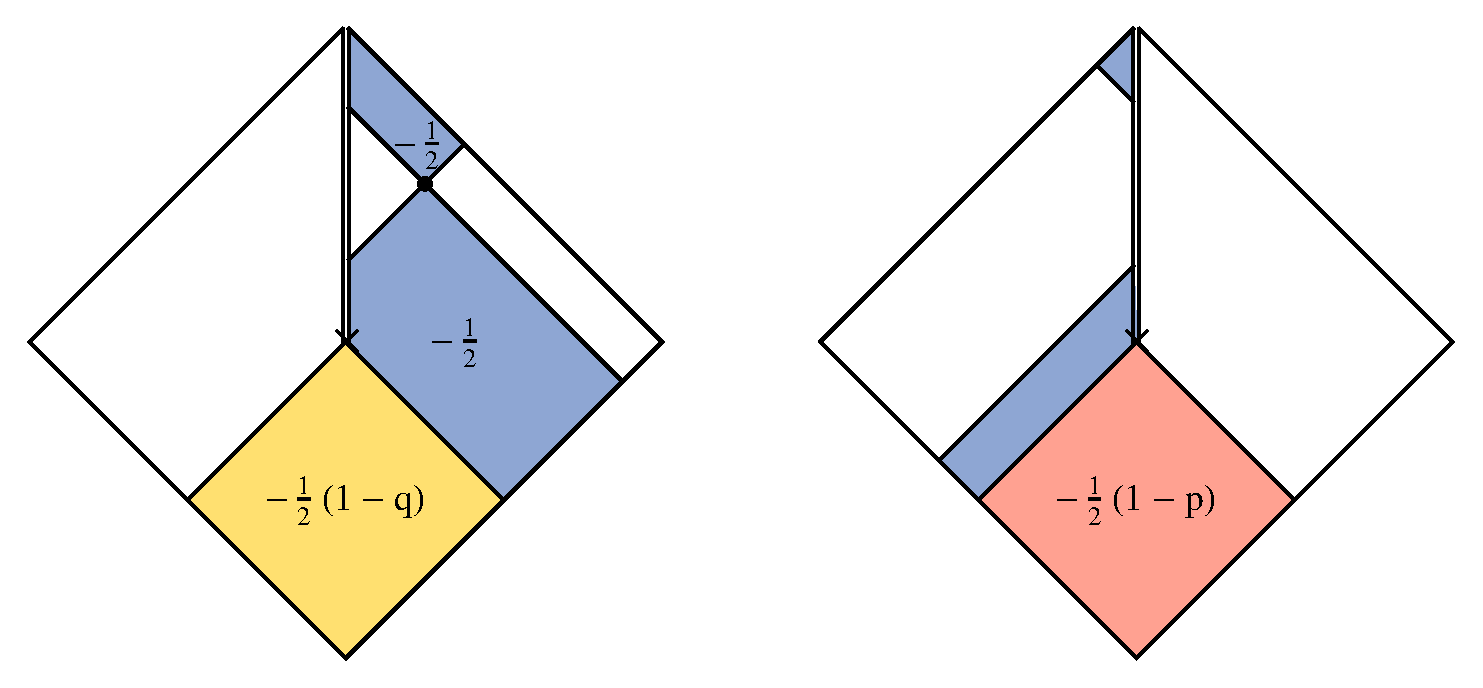
\includegraphics[
clip=true,
width=1.0\textwidth]
{pj-on-pod.pdf}%trim=l b r t, clip=true,
\caption[]{The Pauli-Jordan function $\Delta_p(x,y)$ in the trousers as a function of $y$, with the first argument $x$ fixed (at the dot) in the causal future of the crotch singularity. Here $q=1-p$.}
\label{fig:pj-on-pod}
\end{figure}

\subsection{Counting eigenmodes}
Recall from~\eqref{eq:hsusefulrelation} that if $i\Delta(x,y)$ is a Hilbert-Schmidt integral kernel on $L^2(M\times M)$ with eigenvalues $\lambda_k$ then
\be
\int_M dx\int_M dy |i\Delta(x,y)|^2 = \sum_k\lambda_k^2.
\ee
Let us evaluate the left hand side for $i\Delta_p(x,y)$ on the pair of diamonds. The integral over $y\in\POD$ yields
\be
\int_{\POD}dy|\Delta(x,y)|^2=\frac12(L^2+uv) - \frac12p(1-p)L^2 \Causal(x)
\ee
where $x=(u,v)$. Further integrating this expression over $x\in\POD$ we obtain
\be
\int_\POD dx\int_\POD dy |i\Delta(x,y)|^2 = 2L^4\left[2-p(1-p)\right].
\label{eq:hsnormpod}
\ee
Compare this to the single flat diamond, on which the norm of $i\Delta$ evaluates to $2L^4$. The relation~\eqref{eq:hsnormpod} is useful because it allows us to check if a given set of eigenfunctions of $i\Delta$ is the full set. If the eigenvalues (with multiplicities) sum to less than $2L^4\left[2-p(1-p)\right]$, we know that we are missing eigenfunctions. It is also interesting to note that the value depends on $p$. This means that the eigenvalues must depend on $p$. 
%(the multiplicities $m_k$ are integers so they cannot depend on continuously on $p$).
\begin{figure}
\centering
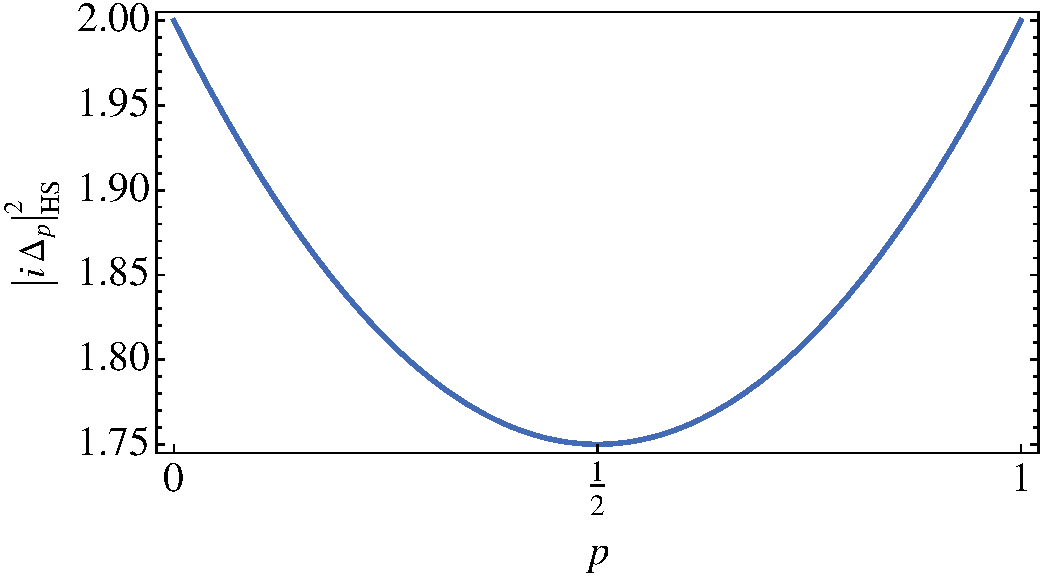
\includegraphics[
clip=true,
width=0.75\textwidth]
{hsnorm-pod.pdf}%trim=l b r t, clip=true,
\caption[]{$L^2(M\times M)$-norm of $i\Delta_p(x,y)$ on the pair of diamonds as a function of $p$.}
\label{fig:hsnorm-pod}
\end{figure}

%
\iffalse
\begin{figure}
\centering
\includegraphics[
clip=true,
width=1.0\textwidth]
{pod-labelled.pdf}%trim=l b r t, clip=true,
\caption[]{The subregions of the pair of diamonds as defined in table~\ref{tab:pod-regions}. The two highlighted regions correspond to Top Left Diagonal 1 (blue, darker) and Bottom Left Diagonal 2 (yellow, lighter).}
\label{fig:pod-regions}
\end{figure}
\fi

\subsection{Ordinary plane waves}
Since we know the SJ modes for the ordinary causal diamond from Chapter~\ref{chapter:diamond}, we can use them as a first guide to guess what eigenmodes might look like on the pair of diamonds.  Recall that on the causal diamond of ``side-length'' $2L$ (i.e. volume $4L^2$) in Minkowski space the Pauli-Jordan function is given by $\Delta(x,y)=-\frac{1}{2}\left[\chi(x\prec y)-\chi(y\prec x)\right]$ and its eigenmodes are linear combinations of positive frequency plane waves and a constant~\eqref{eq:SJfunctions}
\be
\begin{aligned}
f_k(u,v) &:= e^{-iku} - e^{-i k v}, & &\quad\textrm{with } k = \frac{n \pi}{L}, \; n = 1, 2, \ldots\\
g_k(u,v) &:= e^{-iku} + e^{-i k v} - 2 \cos(k L), & &\quad\textrm{with } k\in\mathcal{K}
\end{aligned}\notag\ee
with $\mathcal{K}=\left\{k\in\mathbb{R}\,|\,\tan(kL)=2kL\textrm{ and } k>0\right\}$. Evaluating the action of $i\Delta_p$ on these modes involves rather long calculations on different parts of the pair of diamonds, so
it will be helpful to first consider plane waves that are defined on smaller subregions of the diamond (i.e. that have smaller support).

%(Note that the manipulations that lead from~\eqref{eq:iDeltaULDone} to~\eqref{eq:iDeltaURDone} apply here as well).
%\input{upper-right-mover.tex}


\subsection{Restricted plane waves}
The simplest functions to start with are ``in'' and ``out'' plane waves, which correspond to plane waves that propagate from the trunk into the legs (or from one of the legs into the trunk). Left- and right- propagating plane waves will respectively be functions of $v$ and $u$ only, and therefore it is natural to restrict them to diagonal subregions of the pair of diamonds. We thus consider plane waves $e^{-iku}$ and $e^{-ikv}$. Let us define four types of right-moving plane waves
\bea
U^{R}_k(x)&=e^{-iku}R(x)
\eea
for regions $R=\ULDone,\ULDtwo,\LRDone,\LRDtwo$\, and four types of left-moving plane waves
\bea
V^{L}_k(x)&=e^{-ikv}L(x)
\eea
for regions $L=\URDone,\URDtwo,\LLDone,\LLDtwo$. (Recall that we are using $x=(u,v)$ as a spacetime coordinate.) These functions all solve the wave equation since they are functions of either $u$ or $v$ only (involving only exponentials and step functions in either $u$ or $v$ respectively).

To find the action of $i\Delta_p$ on these functions we need to convolve them with the second argument of $i\Delta_p$ over the pair of diamonds. There is of course perfect symmetry under an exchange of the two diamonds, so it suffices to consider the four modes defined with respect to $D_1$ (i.e. the right-movers on $\ULDone$ and $\LRDone$ and the left-movers on $\URDone$ and $\LLDone$). The actual calculation needs to be done for each subregion of the diamonds separately --- for instance the integral
\be
i\Delta_p U^R_k(x)=\int_{\POD}\sqrt{-g(y)}dy\,i\Delta_p(x,y)U^R_k(y)
\ee
will look different depending on which subregion of the pair of diamonds $x$ lies in due to the functional form of $i\Delta_p$ (see Figure~\ref{fig:pj-on-pod}). For the right-moving plane wave in the upper left diagonal region $\ULDone$ we find
\bea
\frac{k}{L}i\Delta^{}_p U^{\ULDone}_k(x)
&= \ULDone\left(x\right)\left[e^{-iku}+\left(1-\frac{v}{L}\right)\epsilon(kL)-1\right]\\
&\,+\Bone\left(x\right)\left(1-p-\frac{v}{L}\right)\epsilon(kL)\\
&\,+\MRtwo\left(x\right)\left(1-\frac{v}{L}\right)\epsilon(kL)\\
&\,+\Btwo\left(x\right)\,p\,\epsilon(kL)
\label{eq:iDeltaULDone}
\eea
where $\epsilon(kL)=\frac12\left(1-e^{-ikL}\right)$. Given the mirror symmetry of the setup (symmetry under a simultaneous reflection in both diamonds about their vertical axes of symmetry), the expression for the action of $i\Delta_p$ on left-movers in the upper right diagonal region $i\Delta_p V^{\URDone}_k(x)$ can be obtained from~\eqref{eq:iDeltaULDone} by reflecting the regions in each of the two diamonds along the verticals $x_1=x_2=0$ and interchanging $u\leftrightarrow v$ and $p\leftrightarrow 1-p$. This leads to:
\bea
\frac{k}{L}i\Delta^{}_p V^{\URDone}_k(x)
&= \URDone\left(x\right)\left[e^{-ikv}+\left(1-\frac{u}{L}\right)\epsilon(kL)-1\right]\\
&\,+\Bone\left(x\right)\left(p-\frac{u}{L}\right)\epsilon(kL)\\
&\,+\MLtwo\left(x\right)\left(1-\frac{u}{L}\right)\epsilon(kL)\\
&\,+\Btwo\left(x\right)\,\left(1-p\right)\,\epsilon(kL).
\label{eq:iDeltaURDone}
\eea
Analogous expressions can be derived for the lower diagonal right-movers
\bea
\frac{k}{L}i\Delta^{}_p U^{\LRDone}_k(x)
&= \LRDone\left(x\right)\left[e^{-iku}+\left(1+\frac{v}{L}\right)\overline{\epsilon}(kL)-1\right]\\
&\,+\LL\left(x\right)\,\left(1-p\right)\overline{\epsilon}(kL)\\
&\,+\RL\left(x\right)\left(p+\frac{v}{L}\right)\overline{\epsilon}(kL)\\
&\,+\MLone\left(x\right)\left(1+\frac{v}{L}\right)\overline{\epsilon}(kL)
\label{eq:iDeltaLRDone}
\eea
where $\overline{\epsilon}(kL)=\epsilon(-kL)=\frac12\left(1-e^{ikL}\right)$. For the lower diagonal left-movers we obtain
\bea
\frac{k}{L}i\Delta^{}_p V^{\LLDone}_k(x)
&= \LLDone\left(x\right)\left[e^{-ikv}+\left(1+\frac{u}{L}\right)\overline{\epsilon}(kL)-1\right]\\
&\,+\RL\left(x\right)\;p\,\overline{\epsilon}(kL)\\
&\,+\LL\left(x\right)\left(1-p+\frac{u}{L}\right)\overline{\epsilon}(kL)\\
&\,+\MRone\left(x\right)\left(1+\frac{u}{L}\right)\overline{\epsilon}(kL).
\label{eq:iDeltaLLDone}
\eea
We can see that in general, convolution with $i\Delta$ spreads the support of a restricted plane wave onto other regions of the pair of diamonds. A special case is $\epsilon(kL)=0$, which corresponds to $kL=2n\pi$ ($n\in\mathbb N$), for which all but the first lines in the equations above vanish. However, for any single mode there is still an extra constant term on the right hand side and so no single mode will be an eigenfunction of $i\Delta$.

\subsection{Ordinary plane waves revisited}
Given the above results it is easy to find the action of $i\Delta$ on ordinary plane waves via linear combinations of the form $u_k(x)=u^1_k(x)+u^2_k(x)=U^{\LRDone}_k(x)+U^{\ULDone}_k(x) +U^{\LRDtwo}_k(x) +U^{\ULDtwo}_k(x)$. We find that the action of $i\Delta$ on these ordinary plane waves is precisely the same as that for the single diamond if the length scale $L$ on the single diamond is replaced by its direct counterpart $L$ on the pair of diamonds --- the dependence on $p$ drops out. Hence, despite the modified form of the Pauli-Jordan function $i\Delta_p$ on the pair of diamonds it turns out that these modes --- when extended onto both diamonds --- are eigenmodes of $i\Delta_p$, for any value of $p$. Notice that for even $n$, these modes can be viewed as forward-propagated modes on the full trousers (with $L$ equal to $\lambda$), but for odd $n$, they do \emph{not} correspond to such modes. Now, we know from our analysis of the single diamond that the eigenvalues of these modes sum to $2L^4$! Hence we are short by an amount $2L^4\left[1-p(1-p)\right]$ from the total derived in~\eqref{eq:hsnormpod}. We must keep looking.

\subsection{Restricted constant functions}\label{sec:constantmodes}
One of the problems with the general solutions above is that $i\Delta$ acting on a restricted plane wave gives rise to terms that are constant or linear in $u$ or $v$, on regions outside the support of the original function. Perhaps we may hope to find eigenmodes by including constant functions defined on subregions of the pair of diamonds. After all, the single diamond SJ modes included a constant part as well. Note that constant functions can be denoted as multiples of the indicator function. We obtain for $\Bone$:
\bea
&\left(i\Delta_p\Bone\right)(x)
&=&-\frac{i}2L(L+u+v)\Bone(x)\\
&&&-\frac{i}2L^2p\,\RL(x) -\frac{i}2L^2(1-p)\,\LL(x)\\
&&&-\frac{i}2L(L+v)\MLone(x)-\frac{i}2L(L+u)\MRone(x)\\
\eea
for $\MLone$ and $\MRone$:
\bea
&\left(i\Delta_p\MLone\right)(x)
&=&-\frac{i}2L(u+v)\MLone(x)-\frac{i}2Lu\,\LL(x) -\frac{i}2Lv\Bone(x)\\
%
&\left(i\Delta_p\MRone\right)(x)
&=&-\frac{i}2L(u+v)\MRone(x)-\frac{i}2Lv\,\LL(x)-\frac{i}2Lu\Bone(x)\\
\eea
and for $\LL$ and $\RL$:
\bea
&\left(i\Delta_p\LL\right)(x)
&=&\frac{i}2L(L-u-v)\LL(x)+\frac{i}2L^2p\,\Btwo(x) +\frac{i}2L^2(1-p)\,\Bone(x)\\
&&+&\frac{i}2L(L-u)\MLone(x)+\frac{i}2L(L-v)\MRtwo(x)\\
&\left(i\Delta_p\RL\right)(x)
&=&\frac{i}2L(L-u-v)\RL(x)+\frac{i}2L^2p\,\Bone(x) +\frac{i}2L^2(1-p)\,\Btwo(x)\\
&&+&\frac{i}2L(L-v)\MRone(x)+\frac{i}2L(L-u)\MLtwo(x)\\
\eea
Unfortunately, we have not so far been able to find combinations of the functions listed in these sections that are eigenfunctions of $i\Delta_p$. 

\section{Outlook}
In this chapter we have presented the current state of affairs of some initial investigations of the SJ formalism on the trousers spacetime. There are some clear open ends to be tied up, which include, in particular: $(i)$ a derivation of the remaining eigenmodes of $i\Delta$, $(ii)$ an analysis of time-reversibility and of backward-propagated modes, and $(iii)$ a more careful study of the space $L^2(M)$ on the pair of diamonds (and of its complete bases). These points are of course all intertwined and in addressing any one of them we may hope to gain new insight into the others. It is clear that the singularity associated with the topology-change makes the analysis of eigenfunctions more complicated (as, for example, compared to the single diamond). This suggests that one may also try the approach taken in Chapter~\ref{chapter:desitter}, i.e. starting with a complete set of modes and finding the SJ modes by solving for the Bogoliubov coefficients. %For this, we need a complete orthonormal basis for $L^2(\POD)$ (which will necessarily include functions of the type given in Section~\ref{sec:constantmodes}) 

We have also found that the one-parameter family of evolution laws obtained by requiring $\Delta$ to solve the wave equation in the sense of being annihilated by $\mathfrak B$ seems to agree exactly with the family derived in~\cite{Copeland:1988tr}. The approach here has been rather different, but it is not surprising to find that conditions on the regularity of the classical propagators on one hand, and conditions on the conservation of the inner product on the other, lead to the same result. 

%Hence, our evolution law falls foul of the criteria demanded in~\cite{Copeland:1988tr}. It appears that we cannot hope to uphold time-reversibility if we require that $\Delta_p$ solve the wave equation everywhere. We can hope to gain a better understanding of these aspects once we have the full set of eigenmodes of $i\Delta$ and its associated SJ two-point function.


In their conclusion, Copeland et. al. mention ``one more possibility to be considered before accepting the conclusions [on the unphysical nature of the trousers topology-change] of Anderson and DeWitt''. This relates to the fact that in the field expansions used by both Anderson and DeWitt and Copeland et.al., some modes have been ``overlooked'', namely the restricted constant functions of Section~\ref{sec:constantmodes}.
These functions indeed come out naturally when using the one-parameter family of evolution laws compatible with the field equations to propagate plane waves past the singularity (see Section~\ref{sec:proppastsing} above and the Appendix of~\cite{Copeland:1988tr}). In the canonical approach, it is not a priori \emph{necessary} to include these functions in the field expansion, and indeed their inclusion requires the treatment of fundamentally discontinuous modes and their derivatives. In the SJ formalism, however, there seems to be no way to avoid them! Given the comments in the introduction to this chapter, this is not to say that one should expect such issues to cure the pathology of the trousers spacetime --- still, it does raise interesting questions, which we will hopefully be able to answer better in the future.


\end{document}